\documentclass[12pt]{article}

\usepackage{enumerate}
\usepackage[margin=1.5in]{geometry}
\usepackage[pdftex]{graphicx}
\usepackage{amsmath}

\newcommand{\newLine}{\vspace{5mm}}
\newcommand{\appname}{\textit{Pro Quadrature Viewer ZX790}} 
\newcommand{\nextsection}[1]{\newpage\noindent\Large\textbf{#1}\vspace{10mm}\normalsize} 
\newcommand{\nextsubsection}[1]{\newLine \noindent \large \textbf{#1} \normalsize}
\newcommand{\integral}[3]{\text{$\int^{#2}_{#1} #3\,dx$}}
\newcommand{\summation}[3]{\text{$\sum^{#2}_{#1} #3$}}
\newcommand{\floor}[1]{\text{$\lfloor#1\rfloor$}}

\title{Pro Quadrature Viewer ZX790 \\ \Large User's Guide}			
\author{ Jorge Almeyda, John Kluesner, Max Mays}



\begin{document}
\maketitle

\newLine
Welcome to the user's guide for \appname. This application has the power to find the area under a curve of a function efficiently using many different numerical methods. The source code was written in Python using the NUMPY and SCIPY libraries as well as QTDESIGNER for the General User Interface. The numerical methods were cheifly written by Jorge Almeyda and John Kluesner, while the user interface was created by Max Mays. This was the 2-month long project created by the trio for Dr. Robert Olsen's 2013 Spring term Python Computing class at the Richard Stockton College of New Jersey.

\newLine\noindent 
The numerical methods included are (in order of accuracy):
\begin{enumerate}[\indent 1.]
\item Monte Carlo Integration
\item Left Endpoint Riemman Summation
\item Right Endpoint Riemman Summation
\item Composite Trapezoidal Rule
\item Midpoint Riemman Summation
\item Composite Simpsons Rule
\item Gaussian-Legendre Quadrature
\end{enumerate} 
\appname \, has many applications such as: a teaching tool, a way to verify answers for homework problems, or comparing different numerical integration methods in terms of speed and accuracy for a problem you're working on. 


 
\nextsection{Table of Contents}
\begin{enumerate}[\indent 1.]
\item Getting Started 
	\begin{enumerate}[\indent i.]
	\item Using the GUI
	\item Limits and Parameters of the Numerical Methods
	\end{enumerate}
\item Mathematical Background
	\begin{enumerate}[\indent i.]
	\item Monte Carlo Integration
	\item Left Endpoint Riemman Summation
	\item Right Endpoint Riemman Summation
	\item Composite Trapezoidal Rule
	\item Midpoint Riemman Summation
	\item Composite Simpsons Rule
	\item Gaussian-Legendre Quadrature
	\end{enumerate}
\item Limitations and Extensions of \appname
	\begin{enumerate}[\indent i.]
	\item Limitations
	\item Extensions
	\end{enumerate}
\item Sources and Credits
\end{enumerate}



\nextsection{1. Getting Started}

\newLine This section of the user's guide is written for people who just want to get things going and see some results. It's the recommended section to start with and almost a prerequisite to using \appname. If you don't care about the mathematical underpinnings of the numerical methods, then it's the only section you'll need to read. The math is fun though, so you really should at least glaze over it!

\nextsubsection{i. Using the GUI} 

\newLine The \appname interface has been designed for ease of use and dynamic comparison of the various quadrature methods supported by the program. In general, the program is broken up into a few sections:


\nextsubsection{ii. Limits and Parameters of the Numerical Methods}

\newLine  Jorge, this is the section that I want you to write.

This subsection will be written by John and Jorge and will discuss the inputs for each numerical method in a little more detail. It should present the quadrature method in summation form with the error term where applicable (I can just paste that in at the end). It should include a note about the highest degree Polynomial that can be computed perfectly by that method. 

So write something like:

\newLine Left-Endpoint Riemman Summation works by creating rectangles with height at the left-most part of the subinterval to approximate the integral. It follows the followng formula:
\begin{equation*} \integral{a}{b}{f(x)} = h\summation{i = 0}{n - 1}{f(x_i)} + \frac{h}{2}(b-a)f'(\mu), \end{equation*}
where $\mu\in[a,b]$. (Jorge, note that the $n$ in the summation is not the number of subintervals, as defined in the GUI. Think of a simple way to let the reader know that). It can integrate any polynomial of degree 0 perfectly. 
\nextsection{2. Mathematical Background}

This section is for the user who wants to see where these methods come from. A prerequisite to understanding the methods would be Calculus 1 and 2. In particular: definite integrals, derivatives, and Taylor Expansions. 

There are 4 types of numerical integration included in \appname: Stochastic Methods, Composite Newton-Cotes Quadrature, Riemman Summations, and Gaussian Quadrature. 

Stochastic Methods work by using random numbers to approximate a result. They are useful because often times they are iterative in nature. This means that if your current result isn't good enough, you can just do more iterations to get a better result. Their weakness is that they often take more time to get the same results as a more sophisticated method. The Stochastic Method we decided to include is Monte Carlo Integration. 

Composite Newton-Cotes Quadrature Methods work by using evenly spaced intervals to approximate the area under the curve in the form of a summation. That is, they use $\integral{a}{b}{f(x)} \approx \summation{i=k}{n}{c_if(x_i)}$, where each $x_i$ is an equal distance from eachother. The Composite Newton Cotes methods we decided to include are the Trapezoidal Rule and Simpsons Rule. Riemman summations are also special cases of Composite Newton-Cotes Quadrature methods that are presented in most introductory Calculus courses. 

The Gaussian Quadrature method we decided to include is Gaussian-Legendre Quadrature. It's the most common form of Gaussian Quadrature used and it's often the best. It is similar to a Newton Cotes method in that it approximate an integral with a summation, $\integral{a}{b}{f(x)} \approx \summation{i=k}{n}{c_if(x_i)}$, but the difference is the $x_i$'s are often times not equally spaced. It cleverly picks the best $x_i$ values to get best approximation. This allows one to arrive at better approximations with less work.

It should be noted that even though the mathematics presented in this user's guide arrives at the correct results, it abstracts away a lot of mathematical details.

\nextsubsection{i. Monte Carlo Integration}

\newLine One can think of Monte Carlo Integration as randomly throwing a bunch of darts at the graph of a function. The points the darts land at are then compared to the actual value of the function and sees if it's between the curve and the x-axis. Then, the ratio of the area taken up by the curve and the curve's bounding box is approximated by dividing the number of darts between the curve and the x-axis by the total number of darts. From here, we can multiply that ratio by the area of the bounding box to get an approximate area under the curve. Here's an example using 1000 darts to approximate $\integral{0}{4}{\sqrt{4 - (x - 2)^2}}$.


\begin{center}
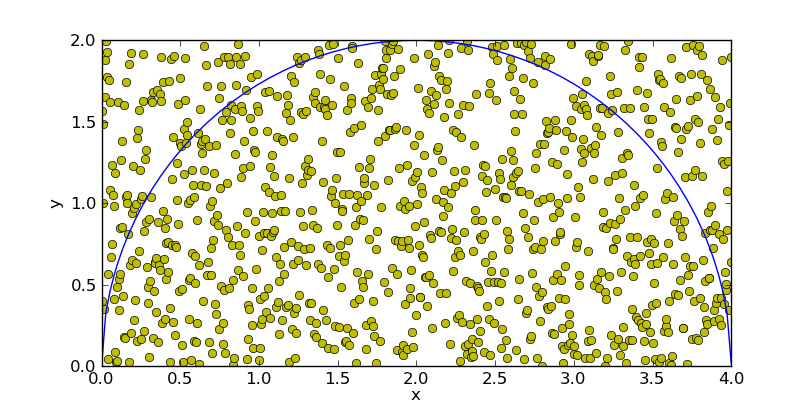
\includegraphics[scale=0.5]{semiCircleMonteCarlo.png}

\small An example of Monte Carlo Integration approximating 

$\integral{0}{4}{\sqrt{4 - (x - 2)^2}}$ with 1000 darts. \normalsize
\end{center}

One can see that using a large number of darts leads to a pretty good approximation of the area under the curve. For further proof, the above example gave the approximate integral of 6.2238414358. The actual value should be half the area of circle with radius of 2, or $2\pi \approx 6.283185307179586$.

Often times, this theory is presented with strictly positive functions. Indeed, that restriction still shows the core theory and understanding of the method. How to apply the same theory to a function that jumps from negative to positive values is a little trickier. Our approach is to do different Monte Carlos Integrations over intervals that are strictly positive and strictly negative. Here's an example that uses 1500 darts to approximate $\integral{0}{8}{(x-2)(x-4)(x-6)(x-8)}$.

\begin{center} 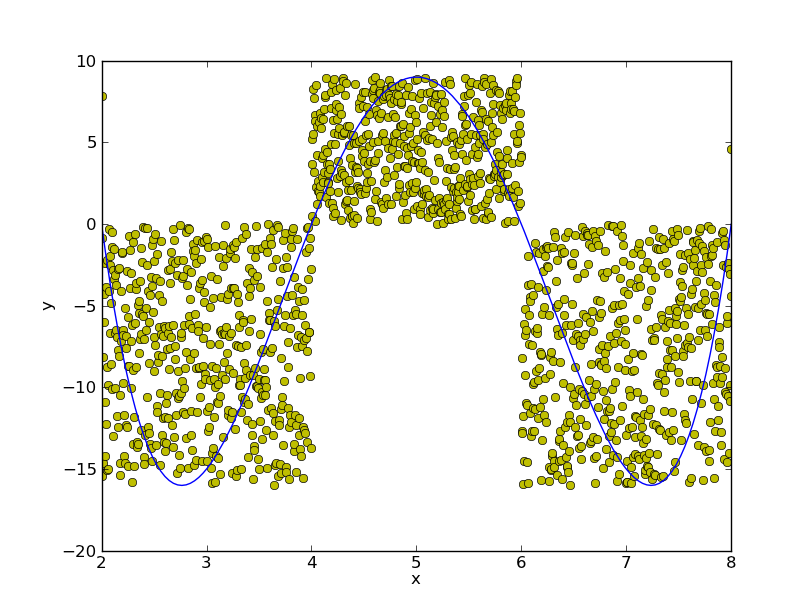
\includegraphics[scale = 0.5]{polynomialMonteCarlo.png} 

\small An example of Monte Carlo Integration approximating $\integral{0}{8}{(x-2)(x-4)(x-6)(x-8)}$ with 1500 darts. \normalsize
\end{center}

\nextsubsection{ii. Left Endpoint Riemman Summation}

\newLine This method is the one that is most often taught in a Calculus 1 course. It approximates the area under the curve by a series of rectangles from the left endpoint of the integral to the right endpoint of the integral. Here's an example of what it looks like when approximating the integral of a logistic equation, $\displaystyle\int^{4}_{-4} \frac{5}{1 +e^{-x}}+1\,dx$.

\begin{center} 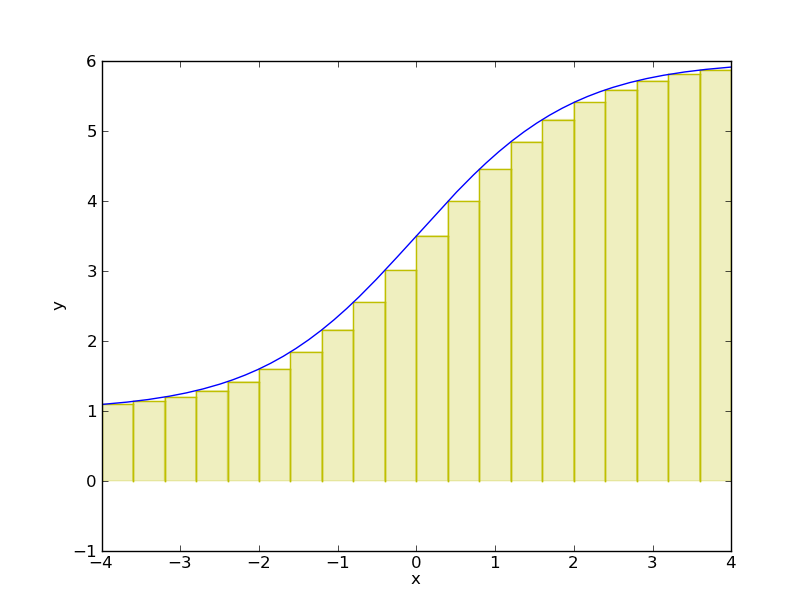
\includegraphics[scale = 0.5]{logisticLeftRiemman.png} 

\small An example of a Left Endpoint Riemman Summation approximating $\int^{4}_{-4} \frac{5}{1 +e^{-x}}+1\,dx$ with 20 rectangles.\normalsize
\end{center}

\noindent Next, we will make a proof outline of The Left Endpoint Riemman Summation to get an error term. First, we approximate our function, $f(x)$, with a Taylor Expansion around the point $x_0 = a$. This gives us

\begin{equation*} f(x) = f(a) + f'(\epsilon)(x - a), \epsilon\in[a,b]. \end{equation*}

\noindent We then integrate the left and right sides from $a$ to $b$ and obtain
\begin{eqnarray*}  \integral{a}{b}{f(x)} &=& \integral{a}{b}{f(a) + f'(\epsilon)(x - a)}  \\
&=& \left. f(a)x + \frac{f'(\epsilon)(x - a)^2}{2}\right|_a^b \\
&=& f(a)(b - a) + \frac{f'(\epsilon)(b - a)^2}{2}
\end{eqnarray*}
If we let the step size, $h = (b - a)$, we get 
\begin{equation*} \integral{a}{b}{f(x)} = hf(a) + \frac{f'(\epsilon)h^2}{2}. \end{equation*}
The term $\frac{f'(\epsilon)h^2}{2}$ is called the remainder term. It can be used to find a bound for the error of the method.

The way we have it set up now is for a single rectangle to approximate the area under the curve, which is obviously a horrible approximation. What we do from there to get to the familar Riemman Sum is split the interval $[a,b]$ into $n$ equally spaced subintervals with the step size $h = \frac{b-a}{n}$. We can denote this in summation form using $x_i = a + ih$ and discarding the error term as
\begin{equation*} \integral{a}{b}{f(x)} = h\summation{i = 0}{n - 1}{f(x_i)}. \end{equation*}
Next, we handle the error term, denoted by $R$. The error term gets summed the same way as above, that is
\begin{equation*} R = \summation{i = 0}{n - 1}{\frac{{f'(\epsilon_i)}h^2}{2}}. \end{equation*}
We define $\mu$ such that $f'(\mu)=\displaystyle\max_{i=0..n-1}(f'(\epsilon_i))$. Then, 

\begin{eqnarray*} R &=& \summation{i = 0}{n - 1}{\frac{{f'(\epsilon_i)}h^2}{2}} \\
&\leq& \summation{i = 0}{n - 1}{\frac{{f'(\mu)}h^2}{2}} \\
&=& n\frac{{f'(\mu)}h^2}{2} \\
&=& \frac{b-a}{h}\cdot\frac{{f'(\mu)}h^2}{2} \\
&=& \frac{h}{2}(b-a)f'(\mu).
\end{eqnarray*}
Thus, our final form for the Left Endpoint Riemman Summation is 
\begin{equation*} 
\integral{a}{b}{f(x)} = h\summation{i = 0}{n - 1}{f(x_i)} + \frac{h}{2}(b-a)f'(\mu).
\end{equation*}

Before you continue, take a closer look at that error term, specifically at $f'(\mu)$. What we want is for the error term to be as close to zero as possible. What we can do is pick a function $f(x)$ such that $f'(x) = 0$. It turns out that one such function is a constant Polynomial, like $f(x) = 5$ or $f(x) = \pi$. This sounds silly now, but what if we could generate a Quadrature method which has an error term of something like $f^{(4)}(\mu)$. That would mean that our Quadrature method could approximate any cubic Polynomial perfectly. It turns out there are many quadrature methods that can do this and we will examine some later. 

\nextsubsection{iii. Right Endpoint Riemman Summation}

\newLine Right Endpoint Riemman Summation is another Quadrature method that is often introduced in a Calculus 1 course. Here's an example for approximating $\integral{-8}{8}{x^2+4}$ with 30 rectangles.

\begin{center} 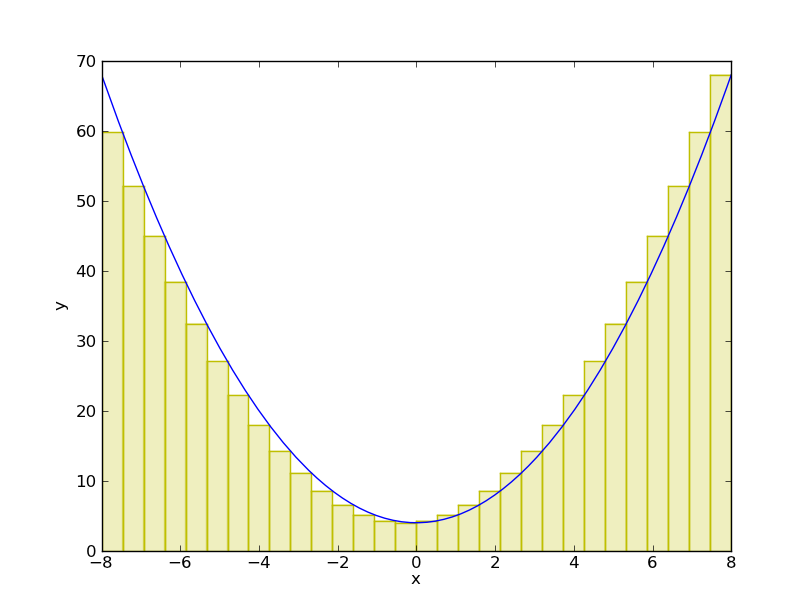
\includegraphics[scale = 0.5]{parabolaRightRIemman.png} 

\small An example of a Right Endpoint Riemman Summation approximating $\integral{-8}{8}{x^2+4}$ with 30 rectangles.\normalsize
\end{center}

Through a similar process to above, we can arrive at the formula
\begin{equation*} 
\integral{a}{b}{f(x)} = h\summation{i = 1}{n}{f(x_i)} - \frac{h}{2}(b-a)f'(\mu),
\end{equation*}

where $x_i = a + ih$ and $\mu\in[a,b]$.

\nextsubsection{iv. Composite Trapezoidal Rule}

\newLine Before we look at the Trapezoidal Rule, let's look back at the formulas for the Right and Left Endpoint Riemman Summations:
\begin{eqnarray*} Q_L(x_i) &=& h\summation{i = 0}{n - 1}{f(x_i)} + \frac{h}{2}(b-a)f'(\mu_L) \\
Q_R(x_i) &=& h\summation{i = 1}{n}{f(x_i)} - \frac{h}{2}(b-a)f'(\mu_R)
\end{eqnarray*}
If we pretend that $\mu_L \approx \mu_R = \mu$, then what would happen if we added them? The remainder terms would cancel out! That means we can go into the next term of the Taylor Expansion and use this new method to approximate any linear Polynomial. We effectively doubled the approximated area though, so a better idea would be to average $Q_L(x_i)$ and $Q_R(x_i)$. Or, if we let $T(x_i)$ be our new approximation:

\begin{eqnarray*} T(x_i) &=& \frac{Q_L(x_i) + Q_R(x_i)}{2} \\
&\approx& \frac{h\summation{i = 0}{n - 1}{f(x_i)} + \frac{h}{2}(b-a)f'(\mu) + h\summation{i = 1}{n}{f(x_i)} - \frac{h}{2}(b-a)f'(\mu)}{2} \\
&=& \frac{h\summation{i = 0}{n - 1}{f(x_i)} + h\summation{i = 1}{n}{f(x_i)}}{2} \\
&=& \frac{h}{2}\left(\summation{i = 0}{n - 1}{f(x_i)} + \summation{i = 1}{n}{f(x_i)}\right) \\
&=& \frac{h}{2}\Big((f(x_0) + f(x_1) + f(x_2) + \cdots + f(x_{n-1})) + (f(x_1) + f(x_2) + \cdots + f(x_{n-1}) + f(x_n))\Big) \\
&=& \frac{h}{2}\Big(f(x_0) + (2f(x_1) + 2f(x_2) + \cdots + 2f(x_{n-1})) + f(x_n)\Big) \\
&=& \frac{h}{2}\Big(f(x_0) + 2\summation{i=1}{n-1}f(x_i) + f(x_n)\Big).
\end{eqnarray*}
This is called the Composite Trapezoidal Rule. The method of getting a better approximation from combining 2 or more worse approximations is called extrapolation and is a very common and useful technique in numerical analysis and mathematics in general. Through another method, we can obtain a remainder term and the general form of the Composite Trapezoidal Rule,

\begin{equation*} 
\integral{a}{b}{f(x)} = \frac{h}{2}\Big(f(x_0) + 2\summation{i = 1}{n-1}{f(x_i)} + f(x_n)\Big) - \frac{h^2}{12}(b-a)f''(\mu).
\end{equation*}
Looking at our remainder term, our intuition was correct and the Composite Trapezoidal Rule indeed approximates any linear polynomial perfectly.

\newLine Additionally, the reason why it's called the Trapezoidal Rule is because it effectively creates trapezoids from adjacent points of the curve to approximate the area. Here's an example for approximating $\integral{-3}{3}{-\frac{x^3}{9}+4}$ with 6 trapezoids:

\begin{center} 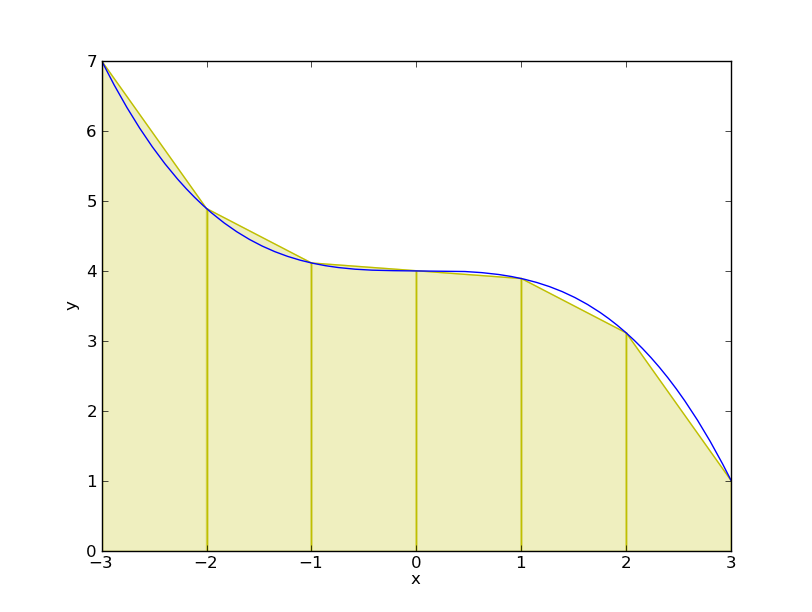
\includegraphics[scale = 0.5]{cubicTrapezoidal.png} 

\small An example of the Composite Trapezoidal Rule approximating 

$\integral{-3}{3}{-\frac{x^3}{9}+4}$ with 6 trapezoids.\normalsize
\end{center}

\nextsubsection{v. Midpoint Riemman Summation}

\newLine The Midpoint Riemman Summation works similarly to the Left and Right Endpoint Summations. It chooses instead to make a rectangle with height from middle of the interval instead of the left or right. Here's an example for approximating $\integral{-\frac{3}{2}\pi}{\frac{3}{2}\pi}{-\cos(x)}$:

\begin{center} 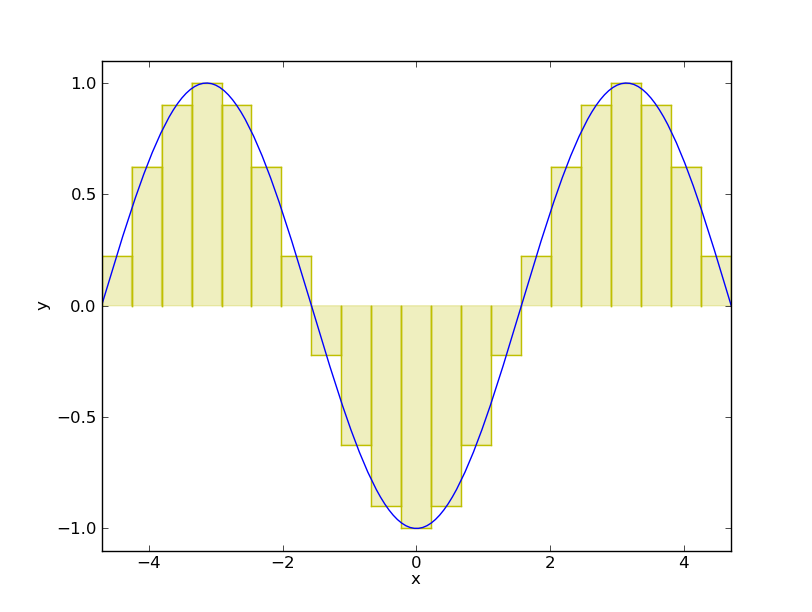
\includegraphics[scale = 0.5]{cosMidpointRiemman.png} 

\small An example of a Midpoint Riemman Summation approximating 

$\integral{-\frac{3}{2}\pi}{\frac{3}{2}\pi}{-\cos(x)}$ with 21 rectangles.\normalsize
\end{center}

Naively, one would think that a Midpoint Riemman Summation would be no better than it's Left or Right Endpoint counterparts. Actually though, it works better than the Composite Trapezoidal Rule. To see why, let's do a proof outline similar to the way we did it with the Left Endpoint Riemman Summation.

First, let's create a Taylor Polynomial expanded around the midpoint of $a$ and $b$, which is $x_0=\frac{a+b}{2}$,

\begin{equation*} f(x) = f(x_0) + f'(x_0)\Big(x - \frac{a+b}{2}\Big) + f''(\epsilon)\frac{(x - \frac{a+b}{2})^2}{2},\end{equation*}
where $\epsilon\in[a,b]$.

\newLine\noindent Note that $b - \frac{a+b}{2}=\frac{b-a}{2}$ and $a - \frac{a+b}{2}=-\frac{b-a}{2}$. Then, we integrate both sides from $a$ to $b$ with respect to $x$,

\begin{eqnarray*} \integral{a}{b}{f(x)} &=& \integral{a}{b}{f(x_0) + f'(x_0)\Big(x - \frac{a+b}{2}\Big) + f''(\epsilon)\frac{(x - \frac{a+b}{2})^2}{2}} \\
&=& \left.f(x_0)x + f'(x_0)\frac{(x - \frac{a+b}{2})^2}{2} + f''(\epsilon)\frac{(x - \frac{a+b}{2})^3}{6}\right|_a^b \\
&=& f(x_0)(b-a) + f'(x_0)\left(\frac{(b - \frac{a+b}{2})^2}{2} -\frac{(a - \frac{a+b}{2})^2}{2}\right) \\
& &\, + f''(\epsilon)\left(\frac{(b - \frac{a+b}{2})^3}{6} - \frac{(a - \frac{a+b}{2})^3}{6} \right) \\
&=& f(x_0)(b-a) + f'(x_0)\left(\frac{(\frac{b-a}{2})^2}{2} -\frac{(-\frac{b-a}{2})^2}{2}\right) \\
& &\, + f''(\epsilon)\left(\frac{(\frac{b-a}{2})^3}{6} - \frac{(-\frac{b-a}{2})^3}{6} \right) \\
&=& f(x_0)(b-a) + f'(x_0)\left(\frac{(\frac{b-a}{2})^2}{2} -\frac{(\frac{b-a}{2})^2}{2}\right) \\
& &\, + f''(\epsilon)\left(\frac{(\frac{b-a}{2})^3}{6} + \frac{(\frac{b-a}{2})^3}{6} \right) \\
&=& f(x_0)(b-a) + f''(\epsilon)\frac{(\frac{b-a}{2})^3}{3}  \\
&=& f(x_0)(b-a) + f''(\epsilon)\frac{(b-a)^3}{24}.
\end{eqnarray*}
From here, we break $b-a$ into $n$ subintervals of size $h=\frac{b-a}{n}$ and define $\mu$ such that $f''(\mu) = \displaystyle\max_{i=0..n-1}f''(\epsilon_i)$  and $x_i = a + \frac{h}{2} + ih$. We wind up with

\begin{eqnarray*} \integral{a}{b}{f(x)} &=& h\summation{i=0}{n-1}{f(x_i)} + \summation{i=0}{n-1}{f''(\epsilon_i)\frac{h^3}{24}} \\
&\leq& h\summation{i=0}{n-1}{f(x_i)} + \summation{i=0}{n-1}{f''(\mu)\frac{h^3}{24}} \\
&=& h\summation{i=0}{n-1}{f(x_i)} + nf''(\mu)\frac{h^3}{24} \\
&=& h\summation{i=0}{n-1}{f(x_i)} + \frac{b-a}{h}\cdot f''(\mu)\frac{h^3}{24} \\
&=& h\summation{i=0}{n-1}{f(x_i)} +  \frac{h^2}{24}(b-a)f''(\mu).
\end{eqnarray*}
Finally, our approximation using a Midpoint Riemman Summation is 

\begin{equation*} \integral{a}{b}{f(x)} = h\summation{i=0}{n-1}{f(x_i)} + \frac{h^2}{24}(b-a)f''(\mu). \end{equation*}

By the remainder term, we can see that it approximates any linear polynomial perfectly. Also, note that the remainder term of the Composite Trapezoidal Rule is twice that of a Midpoint Riemman Summation. This is why a Midpoint Riemman Summation is better than the Composite Trapezoidal Tule theoretically and in practice (try it if you still don't believe me!).

\nextsubsection{vi. Composite Simpsons Rule}

\newLine What the Composite Simpsons Rule does is create a quadratic fit between adjacent sets of three adjacent points. So, if the points to be evaluated by the Composite Simpsons Rule were $x_0,x_1,x_2,x_3,$ and $x_4$, it would create a quadratic fit for $x_0, x_1,$ and $x_2$, and a second one for $x_2,x_3,$ and $x_4$. Here's an example of the Composite Simpsons Rule approximating an integral of a Gaussian Function $\integral{-5}{5}{e^{-\frac{x^2}{2}}}$ with 3 quadratic fits:

\begin{center} 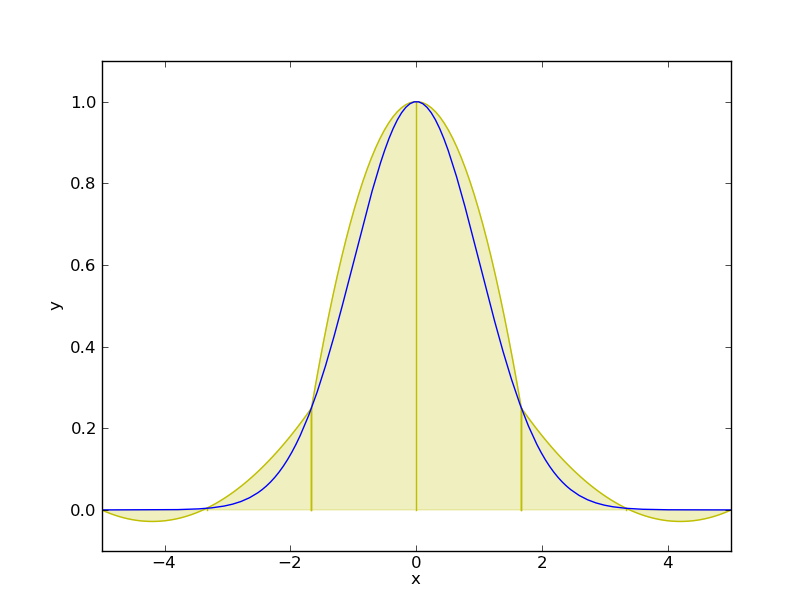
\includegraphics[scale = 0.5]{gaussianSimpsons.png} 

\small An example of the Composite Simpsons Rule approximating 

$\integral{-5}{5}{e^{-\frac{x^2}{2}}}$ with 3 quadratic fits.\normalsize
\end{center}
The formula for the Composite Simpsons Rule will be presented here without any sort of proof outline as it is a little advanced for the target audience of this User's Guide:

\begin{equation*}  \integral{a}{b}{f(x)} = \frac{h}{3}\Big(f(x_0) + 4\summation{i=0}{\floor{\frac{n}{2}}}{f(x_{2i+1})} + 2\summation{i=1}{\floor{\frac{n}{2}}-1}{f(x_{2i})} + f(x_n)\Big) + \frac{h^4}{180}(b-a)f^{(4)}(\mu). 
\end{equation*}
The formula above looks confusing, but all it really is is a complex way of writing
\begin{equation*}  \integral{a}{b}{f(x)} \approx \frac{h}{3}\big(f(x_0) + 4f(x_1)+2f(x_2)+4f(x_3)+\cdots+2f(x_{n-2})+4f(x_{n-1})+f(x_n)\big).
\end{equation*}
Observe that the remainder term has a $4^{th}$ derivative in it, which means Composite Simpson's Rule can approximate any cubic polynomial perfectly.

Note that because the Composite Simpson's Rule needs sets of 3 points to make a quadratic fit, the number of function evaluations has to be odd and the number of subintervals has to be even.

\nextsubsection{vi. Gaussian-Legendre Quadrature}

\newLine Gaussian Quadrature works by using sets of unequally spaced nodes in a quadrature formula. It often times happens that these nodes are more optimal than using equally spaced nodes. The simplest and most optimal points appear from using Gaussian-Legendre Quadrature. Here's a basic outline to generate a Gaussian Quadrature formula for $n=2$.

First, let's look at a the integral of a general cubic polynomial integrated from $-1$ to $1$,
\begin{eqnarray*} \integral{-1}{1}{p(x)} &=& \integral{-1}{1}{c_0 + c_1x + c_2x^2 + c_3x^3} \\
&=& \integral{-1}{1}{c_0} + \integral{-1}{1}{c_1x} + \integral{-1}{1}{c_2x^2} + \integral{-1}{1}{c_3x^3} \\
&=& c_0\integral{-1}{1}{1} + c_1\integral{-1}{1}{x} + c_2\integral{-1}{1}{x^2} + c_3\integral{-1}{1}{x^3}.
\end{eqnarray*}

What that tells us is if we can integrate $1,x,x^2,x^3$ perfectly, then we can integrate any cubic polynomial perfectly. If we try to do this integral with the quadrature formula,
\begin{equation*} \integral{-1}{1}{f(x)} = c_0f(x_0) + c_1f(x_1). \end{equation*}

We can guarentee this quadrature formula will integrate any cubic polynomial perfectly by generating four equations using $f(x)=1,x,x^2,x^3$, like so:

\begin{eqnarray*} \integral{-1}{1}{1} = 2 &=& c_0 + c_1, \\
\integral{-1}{1}{x} = 0 &=& c_0x_0 + c_1x_1, \\
\integral{-1}{1}{x^2} = \frac{2}{3} &=& c_0x_0^2 + c_1x_1^2, \\
\integral{-1}{1}{x^3} = 0 &=& c_0x_0^3 + c_1x_1^3.
\end{eqnarray*}

Observe that we generated 4 equations and 4 unknowns. Therefore, this system can be solved. The algebra will be left to the motivated reader, but the solutions are 
\begin{eqnarray*} c_0 &=& 1, \\
c_1 &=& 1, \\
x_0 &=& \frac{\sqrt{3}}{3}, \\
x_1 &=& -\frac{\sqrt{3}}{3}.
\end{eqnarray*}

This gives us the final formula

\begin{equation*} \integral{-1}{1}{f(x)} = f(\frac{\sqrt{3}}{3}) + f(-\frac{\sqrt{3}}{3}). \end{equation*}.

A good question to ask though is won't this work only for integrals from -1 to 1? The answer to that question is yes, but we can change the limits of integration by a simple linear transformation 
\begin{eqnarray*} z &=& \frac{b-a}{2}x + \frac{b+a}{2}, \\
dz &=& \frac{b-a}{2}dx
\end{eqnarray*}

\noindent Then, we get
\begin{eqnarray*}
\int^a_b f(z)dz &=& \integral{-1}{1}{f(\frac{b-a}{2}x + \frac{b+a}{2})\frac{b-a}{2}} \\
&=& \frac{b-a}{2}\integral{-1}{1}{f(\frac{b-a}{2}x + \frac{b+a}{2})} \\
&=& \frac{b-a}{2}\left(f(\frac{b-a}{2}\cdot\frac{\sqrt{3}}{3}+ \frac{b+a}{2}) + f(-\frac{b-a}{2}\cdot\frac{\sqrt{3}}{3}+ \frac{b+a}{2}) \right)\\
\end{eqnarray*}

This definition makes it obvious that we can generate Quadrature formulas using $n$ nodes to integrate a polynomial of degree $2n-1$ perfectly. 

We can generate all the nodes and coefficients needed as above, but other's have already done that work, so it's more efficient to just take their lists.

\newLine There's another way of viewing Gaussian-Legendre quadrature though, which lends itself much better to the pictorial sense. It turns out that Gaussian-Legendre Quadrature is equivalent to integrating a Polynomial fit that has nodes at the roots of the $n^{\text{th}}$ Legendre Polynomial. That's a much more abstract definition, but it works well for allowing the user to see what Guassian Legendre actually does. Here's an example:

\begin{center}
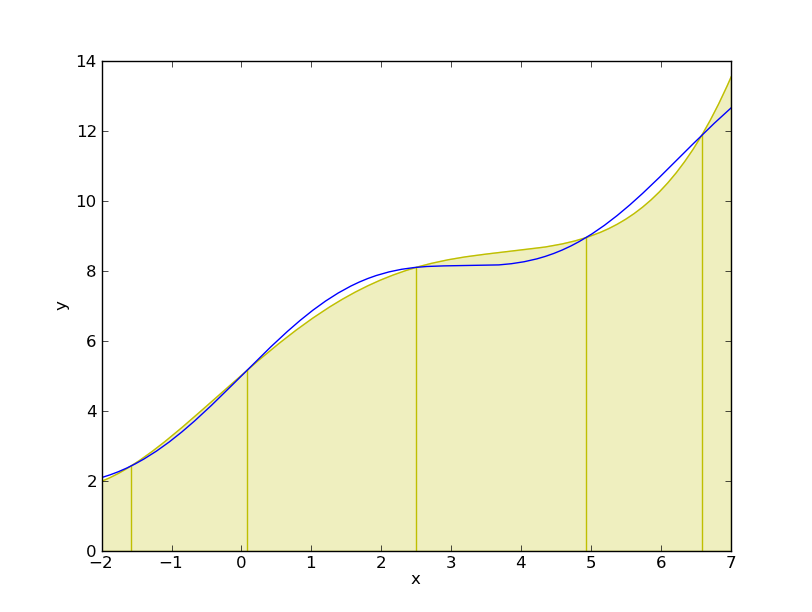
\includegraphics[scale=0.5]{sinXplusXgaussian.png}

\small An example of Gaussian Legendre Quadrature approximating 

$\integral{-2}{7}{\sin{x}+x+5}$ with 5 nodes. \normalsize
\end{center}

\nextsection{3. Limitations and Extensions of \appname}

\appname\, is most certainly a useful tool. We are very proud of our work and think that it would be useful to junior level computational science students to see how approximating the area under a curve works, or a way for students in a introductory numerical analysis course to visualize the quadrature methods they're learning about. There are of course some useful things that it cannot do, and important quadrature methods that are not included.

\nextsubsection{i. Limitations}

\newLine One limitation of \appname\,  is that it only approximates integrals of 1 dimension. It turns out that approximating 2 dimensional integrals is pretty much just using the formula twice, once over each dimension. This is not something that can be done by \appname\, though. Any introductory book on numerical analysis will go over it in more detail for the curious reader.

\newLine A bigger limitation though is that we don't have an option for the user to input a tolerance and have \appname\, go until that tolerance is met and display the $n$ that was needed. The reason we don't have this is because our code works by using NUMPY's array arithmetic. This is a much faster way of doing the quadrature methods than using an explicit for-loop. If we wanted to allow the user to enter a tolerance, that would require an explicit for-loop, which would be very slow. There is something called Adaptive Quadrature though that will approximate the integral to a certain tolerance and still uses array arithmetic. This wasn't included because it creates in own $n$ value based on relative errors and it would make it hard to compare to the other methods.

\nextsubsection{ii. Extensions}

\newLine This section will comprise of a list of popular quadrature methods, a very brief explanation, and a link to a better explanation:

\newLine Clenshaw-Curtis quadrature works by creating a discrete cosine transform and integrating term-by-term. 

\newLine\noindent A python implementation: 

\texttt{\small http://www.scientificpython.net/1/post/2012/04/clenshaw-curtis-quadrature.html \normalsize}

\newLine \newLine Adaptive Simpsons Rule works by choosing the nodes selectively based on how much of the area under the curve it takes up.

\newLine\noindent The quadrature section at this link describes the theory and a MATLAB implementation:

\texttt{\small http://www.mathworks.com/moler/chapters.html \normalsize}

\newLine\newLine Other types of Gaussian Quadrature are better suited to specific types of functions or integrals. For example, Gaussian-Laguerre Quadrature for improper integrals:

\newLine \noindent Wikipedia shows many types of Gaussian Quadrature methods with their nodes and weights:

\texttt{\small http://en.wikipedia.org/wiki/Gaussian\_quadrature \normalsize}

\end{document}